\documentclass{article}
\usepackage{graphicx}
\usepackage{listings}
\usepackage{amsmath}
\begin{document}

\section{Using Figure 2.4 as a model, illustrate the operation of merge sort on the array A=(3,41,52,26,38,57,9,49).}
\begin{figure}[!htb] 
  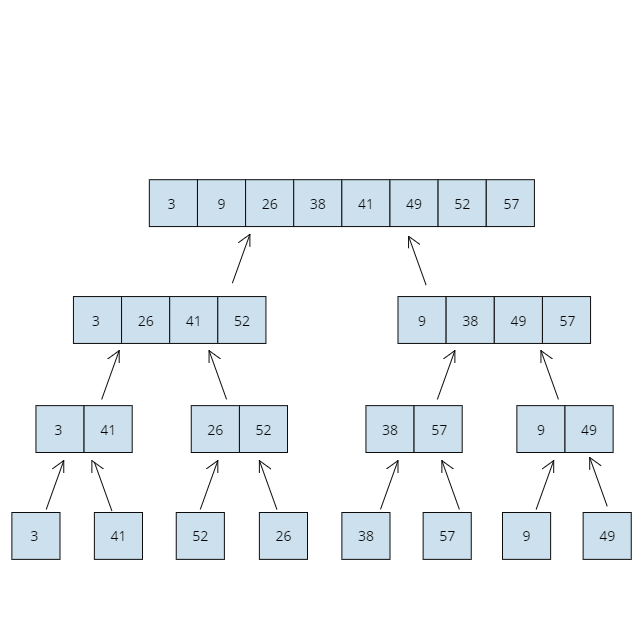
\includegraphics[width=\textwidth]{2_3-1.png}
\end{figure}


\section{Rewrite the Merge grocedure so that it does not use sentinels? instead stopping pnce either array L or Rhas had all elements copied back to A and then colying the remainder of the other array back into A}
\lstinputlisting[language=Python]{2.3-2/merge-sort.py}

\section{2.3-3}
Use mathematical induction to show that when $n$ is an exact power of 2, the solution of the recurrence

$T(n) = 
\begin{cases}
 2, & \mbox{if  $n= 2$} \\
 2T(n/2)+n, & \mbox{if $ n=2^k$, for $k > 1$} 
\end{cases}$ 

is $ T(n) = nlg(n)$

For $n=2$:
$T(2)=2=2lg(2)=nlg(n)$

For $n=4$:
$T(4)=2T(2)+4=2*2lg(2)+4*1=4*lg(2)+4*lg(2)=4*lg(4)=nlg(n)$

Assume, that for all $n \le k$ T(n)=nlg(n).
For $n = k*2$: $T(k*2)=2T(k*2/2)+ 2k=2k*lg(k)+2k=2k*lg(k) +2k*lg2=2k*(lgk + lg2)=2k*lg(2k)$

\section{2.3-4}
We can express insertion sort as a recursive procedure as follows. In order to sort A[1..n], we recursively sort A[1..n-1] and than insert A[n] into the sorted array A[1..n-1]. Write a recurrence for the worst-case running time of this recursive version of insertion sort.

$T(n) = 
\begin{cases}
 \Theta(1), & \mbox{if  $n= 1$} \\
 T(n-1)+n-1, & \mbox{if $n > 1$} 
\end{cases}$ 


\end{document}